\documentclass[floatfix,nofootinbib,superscriptaddress,fleqn]{revtex4-2} 
%\documentclass[aps,epsfig,tightlines,fleqn]{revtex4}
\usepackage[utf]{kotex}
\usepackage[HWP]{dhucs-interword}
\usepackage[dvips]{color}
\usepackage{graphicx}
\usepackage{bm}
%\usepackage{fancyhdr}
%\usepackage{dcolumn}
\usepackage{defcolor}
\usepackage{amsmath}
\usepackage{amsfonts}
\usepackage{amssymb}
\usepackage{amscd}
\usepackage{amsthm}
\usepackage[utf8]{inputenc}
 \usepackage{setspace}
 \usepackage{tikz}
%\pagestyle{fancy}

\begin{document}

\title{\Large 2022년 1학기 물리학 I: Quiz 14}
\author{김현철\footnote{Office: 5S-436D (면담시간 매주
    화요일-16:00$\sim$20:00)}} 
\email{hchkim@inha.ac.kr}
\author{Hui-Jae Lee} 
\email{hjlee6674@inha.edu}
\affiliation{Hadron Theory Group, Department of Physics, Inha
  University, Incheon 22212, Republic of Korea }
\date{Spring semester, 2022}

\vspace{1.cm}

\maketitle

\noindent {\bf 문제 1. (30 pt)} 
그림~\ref{fig:1}에서 크기가 10 N인 힘이 질량 10 kg이고 반지름이 0.30
m인 바퀴에 수평방향으로 작용하고 있다. 바퀴는 수평면에 대하여 유연한
굴림 운동을 하며 질량중심에 대한 가속도의 크기는 0.60
$\mathrm{m/s^2}$이다. 
\begin{figure}[htp]
  \centering
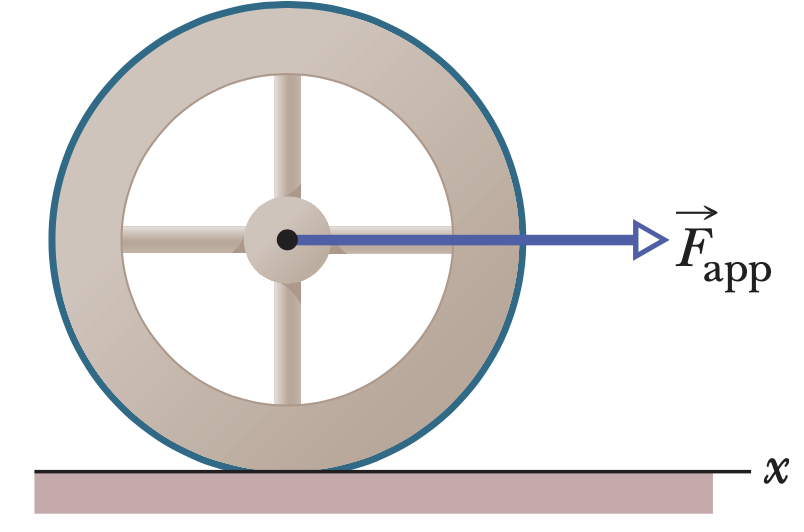
\includegraphics[scale=0.5]{Qfig14-1-20220427.png}
  \caption{문제 1}
  \label{fig:1}
\end{figure}
\begin{itemize}
\item[(가)] 바퀴에 작용하는 마찰력을 단위벡터로 표기하여라.
\item[(나)] 질량중심을 지나는 회전축에 대한 바퀴의 회전관성은
  얼마인가?   
\end{itemize}

\noindent {\bf 풀이 : }
\begin{itemize}
  \item[(가)] 바퀴가 회전하도록 하는 힘은 바퀴에 작용하는 마찰력이다.
  이 마찰력을 $F_s$라 하자.
  바퀴의 질량을 $m$, 반지름을 $r$, 바퀴 중심에 대한 바퀴 끝 부분의 가속도를 
  $a$라 하면
  각가속도 $\alpha$와, 돌림힘 $\tau$를 다음과 같이 표현할 수 있다.
  \begin{align}
    \alpha=\frac{a}{r},\,\,\, \tau = F_s r = I\alpha.
  \end{align}
  마찰력은 바퀴가 움직이는 방향의 반대방향으로 작용하므로,
  \begin{align}
    \vec{F}_s = -\frac{I\alpha}{r}\hat{\bm i}.
  \end{align}
  \item[(나)]
  바퀴의 운동 방정식은 다음과 같다.
  \begin{align}
    \sum F = ma = F_{app} - F_s.
  \end{align}
  마찰력은,
  \begin{align}
    F_s=\frac{I\alpha}{r} = \frac{Ia}{r^2} = F_{app}-ma.
  \end{align}
따라서 회전관성 $I$는 다음과 같다.
\begin{align}
  I = \frac{(F_{app}-ma)r^2}{a}
\end{align}
  수치를 대입하면,
  \begin{align}
    \begin{split}
      I &= \frac{(10\,\mathrm{N} - (10\,\mathrm{kg})(0.60\,\mathrm{m/s^2}))
      (0.30\,\mathrm{m})^2}{(0.60\,\mathrm{m/s^2})} \\
      &=0.6\,\mathrm{kg\cdot m^2}.
    \end{split}
  \end{align}
\end{itemize}

\vspace{1.cm}

\noindent {\bf 문제 2. (30 pt)}
그림~\ref{fig:2}는 질량이 $m$, 반지름이 $R$인 원형고리와 질량이 $m$,
길이 $R$인 네 개의 가느다란 막대로 만들어진 정사각형 강체이다. 강체는
주기가 2.5 초인 일정한 속력으로 수직축에 대하여 회전한다. $R=0.50$ cm,
$m=2.0$ kg이라고 할 때,
\begin{figure}[ht]
  \centering
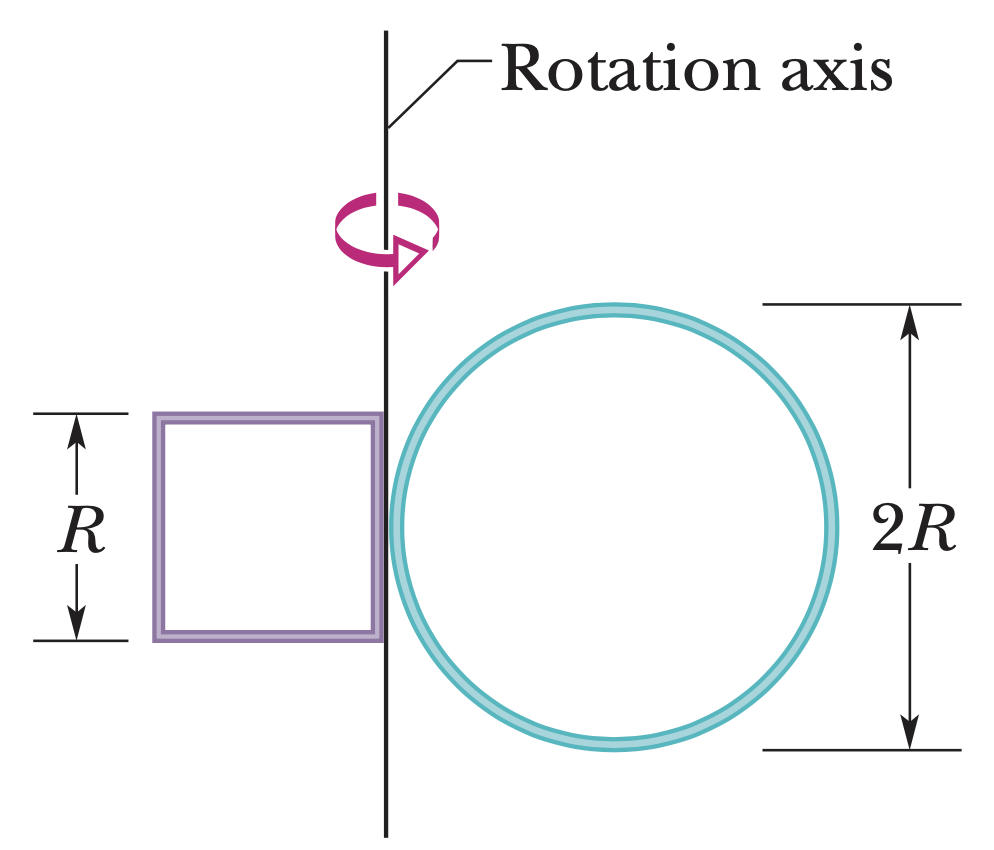
\includegraphics[scale=0.4]{Qfig14-2-20220427.png}
  \caption{문제 2}
  \label{fig:2}
\end{figure}
\begin{itemize}
\item[(가)] 회전축에 대한 강체의 회전관성과
\item[(나)] 회전축에 대한 각운동량을 각각 구하여라.   
\end{itemize}

\noindent {\bf 풀이 : }
\begin{itemize}
  \item[(가)] 
  정사각형일 경우 회전축에 수평한 막대, 수직인 막대를 나누어 생각하자. 
  $\rho$를 고리의 밀도라 하면 수평한 막대의 회전관성 $I_{p}$는,
  \begin{align}
    \begin{split}
      I_{p} = \int r^2\,dm = \rho\int_0^R R^2\,dz + 0 = \rho R^3.  
    \end{split}
  \end{align}
  수직인 막대의 회전관성 $I_{o}$는 다음과 같다.
  \begin{align}
    \begin{split}
      I_{0} = \int r^2\,dm = \rho\int_0^R r^2\,dr+\rho\int_0^R r^2\,dr
      =\frac{2}{3}\rho R^3. 
    \end{split}
  \end{align}
  정사각형 고리의 회전관성은 $I_{p}$ 와 $I_{o}$ 를 합한 것이므로,
  \begin{align}
    I_{p}+I_{0} = \frac{5}{3}\rho R^3 
    = \frac{5}{3}\left(\frac{m}{R}\right) R^3
    =  \frac{5}{3}mR^2.
  \end{align}
  평행축 정리를 이용하여 원형고리의 회전관성을 구하자. 평행축 정리는 다음과 같다.
  $I$는 축을 이동한 후의 회전관성이고 $I_{cm}$은 축을 이동하기 전의 회전관성이다. 
  \begin{align}\label{eq:2-1}
    I = I_{cm}+mh^2.
  \end{align}
  원형고리의 회전관성 $I_{cir}$은,
  \begin{align}
    I_{cir} = I_{cm}+mR^2
  \end{align}
  원형고리일 경우 밀도 $\rho$는,
  \begin{align}
    \rho = \frac{m}{2\pi R}.
  \end{align}
  미소질량 $dm^\prime$을 생각하면,
  \begin{align}
    dm^\prime = \rho R\,d\theta = \frac{m}{2\pi}\,d\theta.
  \end{align}
  $\theta$는 축과 중심을 잇는 선, 중심과 $dm^\prime$을 잇는 선이 이루는 각이다.
  구면좌표계에서 $z$축과 이루는 각도를 생각하면 된다. $r$은 미소질량과 회전축 사이 
  거리이므로 $r=R\sin\theta$ 이다. 따라서 $I_{cm}$은,
  \begin{align}
    \begin{split}
      I_{cm} &= \int r^2\,dm^\prime = \frac{m}{2\pi}R^2
      \int_0^{2\pi}\sin^2\theta\,d\theta
      = \frac{m}{2\pi}R^2\pi = \frac{1}{2}mR^2.
    \end{split}
  \end{align}
  식 \eqref{eq:2-1}에 의해 $I_{cir}$은 다음과 같다.
  \begin{align}
    \begin{split}
      I_{cir} = \frac{1}{2}mR^2+mR^2 = \frac{3}{2}mR^2.
    \end{split}
  \end{align}
  총 회전관성 $I$는 정사각형 고리의 회전관성과 원형고리의 회전관성을 합한 것이므로,
  \begin{align}
    I = I_p+I_o+I_{cir} = \frac{5}{3}mR^2+\frac{3}{2}mR^2=\frac{19}{6}mR^2.
  \end{align}
  수치를 대입하자.
  \begin{align}
    \begin{split}
      I&=\frac{19}{6}(2.0\,\mathrm{kg})(0.50\,\mathrm{cm})^2  \\
      &= 1.6\,\mathrm{kg\cdot cm^2} \\
      &= 1.6\times 10^{-4}\,\mathrm{kg\cdot m^2} .
    \end{split}
  \end{align}
  \item[(나)] 
  정의에 따르면 각속도 $\omega$는,
  \begin{align}
    \omega = \frac{2\pi}{T}.
  \end{align}
  각운동량 $L$은 다음과 같다.
  \begin{align}
    L = I\omega = \frac{2\pi I}{T} = \frac{19\pi mR^2}{3T}.
  \end{align}
  수치를 대입하여 값을 구해보면 다음과 같다.
  \begin{align}
    \begin{split}
      L &=\frac{19\pi (2.0\,\mathrm{kg})(0.50\,\mathrm{cm})^2}
      {3(2.5\,\mathrm{s})}  \\
      &= 4.0\,\mathrm{kg\cdot cm^2/s} \\
      &= 4.0\times 10^{-4}\,\mathrm{kg\cdot m^2/s}.
    \end{split}
  \end{align}
  \end{itemize}

\vspace{1.cm}


\noindent {\bf 문제 3. (40pt)} 
질량이 4.0 kg이고 길이가 0.50 m인 가늘고 균일한 막대가 수평면에서
중심을 지나는 수직축에 대하여 회전할 수 있다. 질량이 3.0 g인 총알이
막대의 회전면에서 정지하고 있는 막대의 왼쪽 끝을 향하여
발사되었다. 위에서 보았을 때 총알의 경로는 그림~\ref{fig:3}처럼 막대와
$\theta=60^\circ$의 각도를 이룬다. 총알이 막대에 박히고 충돌 직후
막대의 가속도가 10 rad/s이라면 충돌 직전 총알의 속력은 얼마인가? 
\begin{figure}[ht]
  \centering
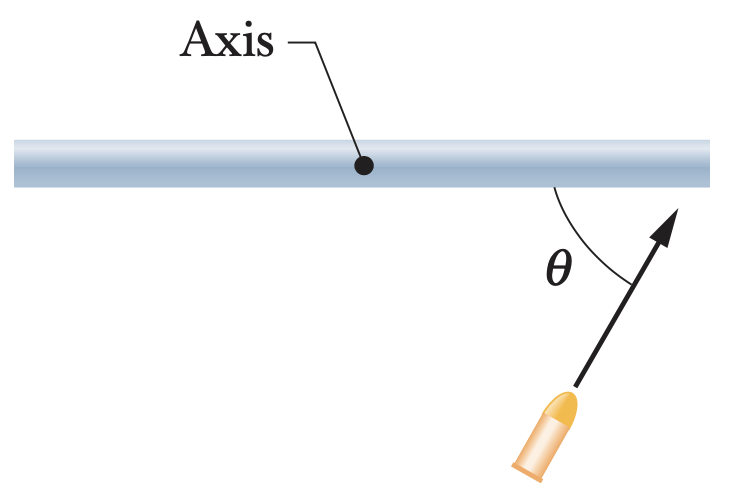
\includegraphics[scale=0.4]{Qfig14-3-20220427.png}
  \caption{문제 3}
  \label{fig:3}
\end{figure}

\noindent {\bf 풀이 : }
$\vec{r}$과 $\vec{p}$는 충돌 직전 회전축에 대한 총알의 위치와 운동량이다.
 총알의 질량을 $m_2$ 총알의 속력을 $v_2$라 하자.
총알이 충돌하기 직전의 각운동량 $L_1$은 다음과 같다.
\begin{align}
  L_1 =|\,\vec{r}\times\vec{p}\,|=\frac{1}{2} m_2v_2d\sin\theta.
\end{align}
나중 각운동량 $L_2$은,
\begin{align}\label{eq:3-1}
  L_2 = I_1\omega+ I_2\omega.
\end{align}
$I_1$은 막대의 회전관성, $I_2$는 총알의 회전관성이다.
막대 질량을 $m_1$, 막대 길이를 $d$라 하면 $I_1$은,
\begin{align}
  I_1 = \int r^2\,dm = \rho\int_{-\frac{1}{2}d} ^{\frac{1}{2}d}r^2\,dr
  =\left(\frac{m_1}{d}\right)\left(\frac{1}{24}d^3
  -\left(-\frac{1}{24}d^3\right)\right)
  =\frac{1}{12}m_1d^2.
\end{align}
$I_2$는,
\begin{align}
  I_2 =  mr^2 = \frac{1}{4}m_2d^2.
\end{align}
식 \eqref{eq:3-1}에 의해 $L_2$는,
\begin{align}
  L_2 = \left(\frac{1}{12}m_1+\frac{1}{4}m_2\right)\omega d^2.
\end{align}
각운동량 보존 법칙에 따르면 $L_1=L_2$이다. 따라서,
\begin{align}
  \frac{1}{2}m_2v_2d\sin\theta=\left(\frac{1}{12}m_1
  +\frac{1}{4}m_2\right)\omega d^2.
\end{align}
$v_2$에 대해 정리해보면 다음과 같다.
\begin{align}
  v_2 = \left(\frac{1}{6}m_1+\frac{1}{2}m_2\right)\frac{\omega d}{m_2\sin\theta}
\end{align}
수치를 대입하여 총알의 속력을 구할 수 있다.
\begin{align}
  \begin{split}
    v_2 &= \left(\frac{1}{6}(4.0\,\mathrm{kg})
    +\frac{1}{2}(3.0\times 10^{-3}\,\mathrm{kg})\right)
    \frac{(10\,\mathrm{rad/s}) (0.50\,\mathrm{m})}
    {(3.0\times 10^{-3}\,\mathrm{kg})\sin{60^\circ}}  \\
    &= 1.3\times 10^3\,\mathrm{m/s}.
  \end{split}
\end{align}
총알의 속력은 $1.3\times 10^3\,\mathrm{m/s}$이다.
\vspace{1.cm}


\noindent {\bf 문제 4. (60pt) {\color{red} 난이도 상}:}
그림~\ref{fig:4}에서 질량 $30\,\mathrm{kg}$의 아이가 질량이 $100\,\mathrm{kg}$, 반지름이 
$2.0\,\mathrm{m}$인 정지해 있는 원판의 가장자리에 서 있다. 원판의 중심에 있는 회전축에
대한 회전관성은 $150\,\mathrm{kg\cdot m^2}$이다. 이때 친구가 던진
질량이 $1.0\,\mathrm{kg}$인 공을 아이가 잡았다. 공을 잡기 직전에 수평방향인 공의
속도 $\vec{v}$의 크기는 $12\,\mathrm{m/s}$이고 원판의 가장자리의 접선과
$\vec{v}$가 이루는 각도는 $37^\circ$이다. 아이가 공을 잡은 직후 원판의
각속력을 구하여라. 
\begin{figure}[ht]
  \centering
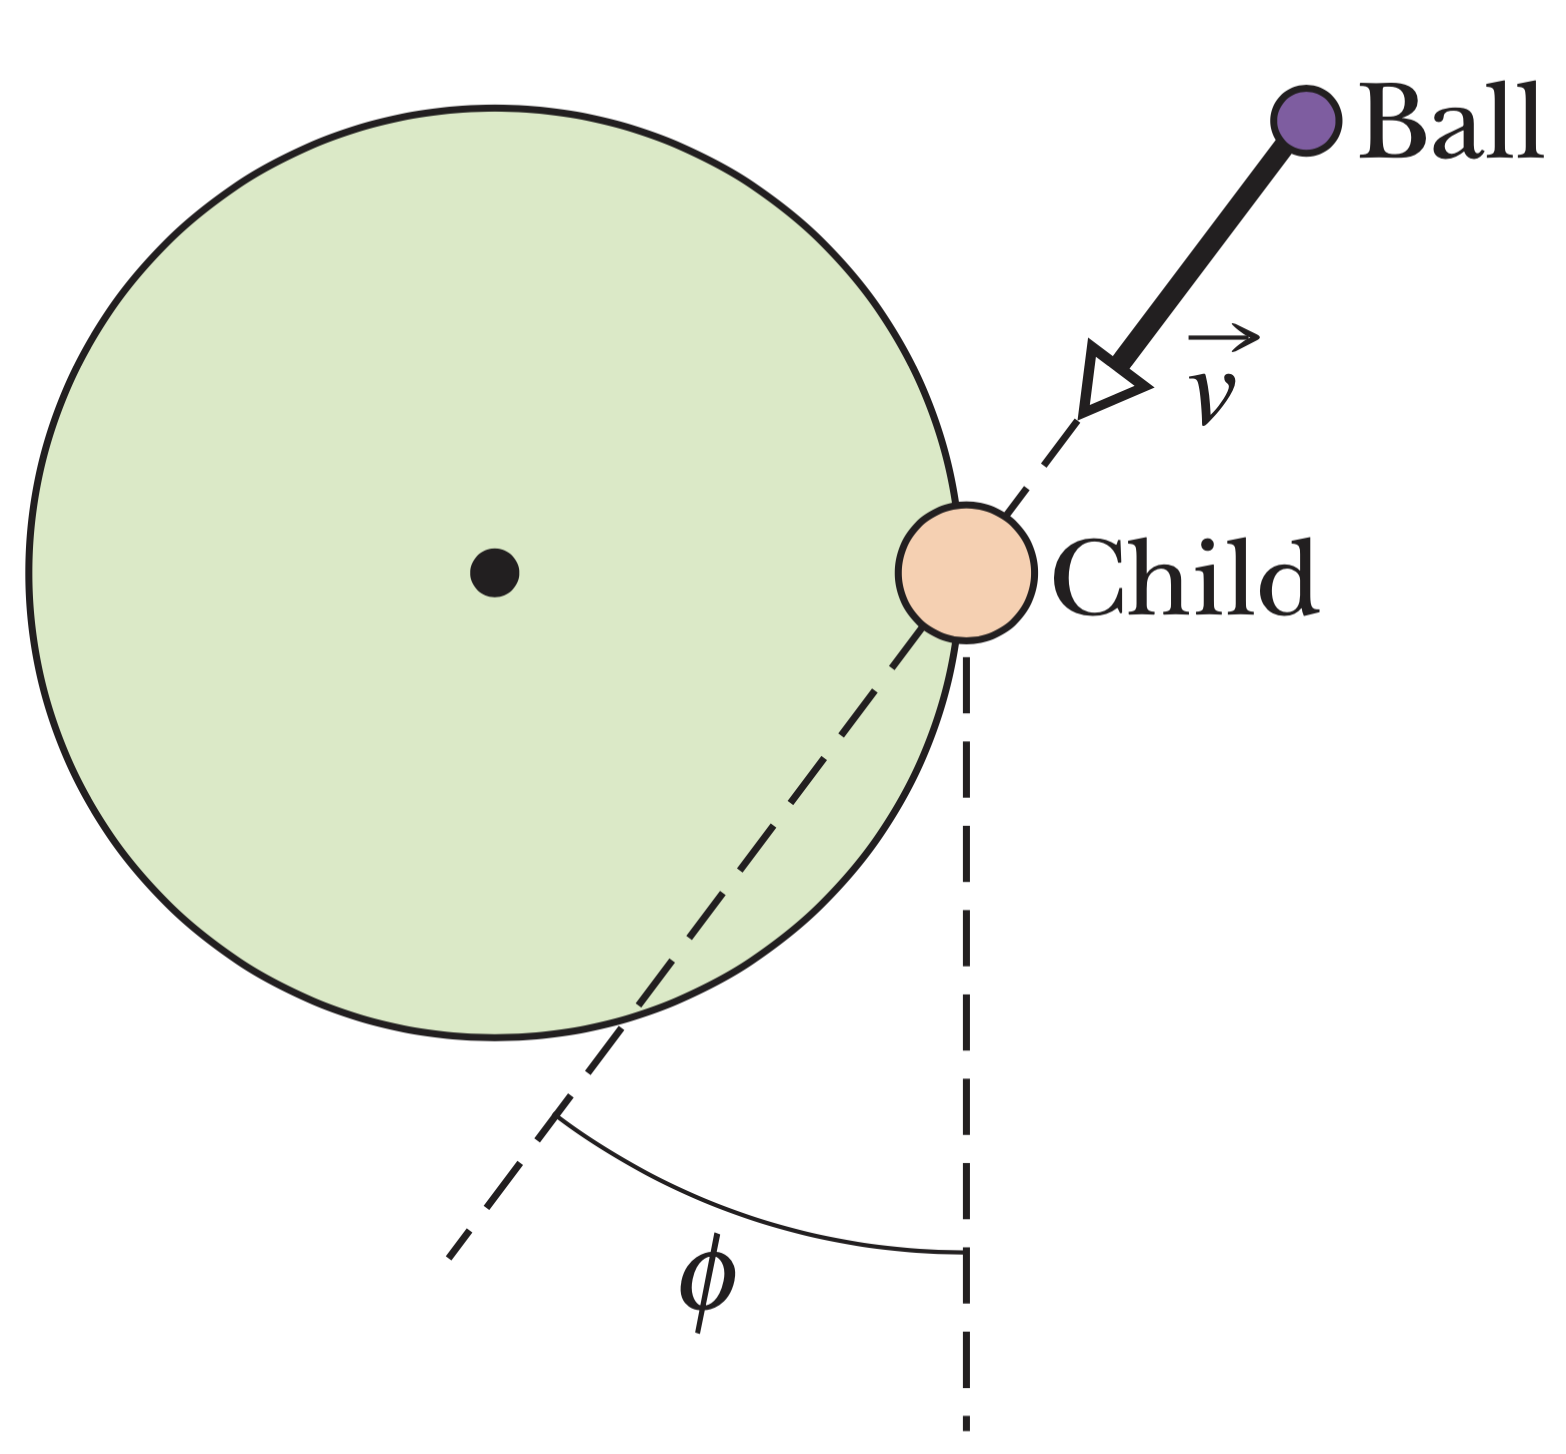
\includegraphics[scale=0.25]{Qfig14-4-20220427.png} 
  \caption{문제 4}
  \label{fig:4}
\end{figure}

\noindent {\bf 풀이 : }
$\vec{r}$과 $\vec{p}$는 아이가 공을 잡기 직전 회전축에 대한 공의 위치와 운동량이다.
원판 반지름을 $R$, 
공 질량과  공 속력을 $m_3$, $v_3$라고 하면 공을 잡기 직전의 각운동량 $L_i$는,
\begin{align}
  L_i =|\,\vec{r}\times\vec{p}\,|
  = m_3v_3R\sin\left(270^\circ-\phi\right).
\end{align}
공을 잡은 후 각운동량을 $L_f$라 하면,
\begin{align}
  L_f = I\omega.
\end{align}
$I$는 계의 총 회전관성이다. 즉, 원판, 아이, 공의 회전관성을 더한 것이 된다.
아이의 질량을 $m_2$라 할 때 
공을 잡은 후 아이와 공의 회전관성 $I_2$는,
\begin{align}
  I_2 = mr^2 = (m_2+m_3)R^2.
\end{align} 
원판의 회전관성을 $I_1$라 하자. 전체 회전관성 $I$는,
\begin{align}
  I = I_1 + I_2 = I_1+(m_2+m_3)R^2.
\end{align}
따라서 공을 잡은 후 각운동량 $L_f$는 다음과 같다.
\begin{align}
  L_f = I\omega = (I_1+(m_2+m_3)R^2)\omega.
\end{align}
각운동량 보존 법칙에 의해 $L_i = L_f$이므로,
\begin{align}
  m_3v_3R\sin\left(270^\circ-\phi\right)
  =(I_1+(m_2+m_3)R^2)\omega.
\end{align} 
각속도 $\omega$를 구해보자.
\begin{align}
  \begin{split}
    \omega &= \frac{m_3v_3R}{I_1+(m_2+m_3)R^2}
    \sin\left(270^\circ-\phi\right)  \\
    &= \frac{(1.0\,\mathrm{kg})(12\,\mathrm{m/s})(2.0\,\mathrm{m})}
    {(150\,\mathrm{kg\cdot m^2})
    +((30\,\mathrm{kg})+(1.0\,\mathrm{kg}))(2.0\,\mathrm{m})^2}
    \sin 233^\circ \\
   &=-0.070\,\mathrm{rad/s}
  \end{split}
\end{align}
따라서 각속력은 $0.070\,\mathrm{rad/s}$이다.
\vspace{1.cm}


\end{document}